% % % % % % % % % % % % % % % % % % % % % % % % % % % % % % % % % % % % % % % % % % % %
%                                                                                     %
% Short Sectioned Assignment LaTeX Template Version 1.0 (5/5/12)                      %
% This template has been downloaded from: http://www.LaTeXTemplates.com               %
%                                                                                     %
% Original author:  Frits Wenneker (http://www.howtotex.com)                          %
%                                                                                     %
% Modified by: Fco Javier Sueza Rodríguez (fcosueza@disroot.org)                      %
%                                                                                     %
% Changes:                                                                            %
%	    - Custom Chapters, Sections and Subsections (titlesec package)                %
%           - Document type scrbook (oneside)                                         %
%           - Use babel-lang-spanish package and marvosym                             %
%           - Use hyperref, enumitem, tcolorbox and glossaries packages               %
%           - Use Time New Roman (mathptmx), Helvetic and Courier fonts               %
%                                                                                     %
% License: CC BY-NC-SA 3.0 (http://creativecommons.org/licenses/by-nc-sa/3.0/)        %
%                                                                                     %
% % % % % % % % % % % % % % % % % % % % % % % % % % % % % % % % % % % % % % % % % % % %

%-----------------------------------------------%
%	              Packages                  %
%-----------------------------------------------%

\documentclass[paper=a4, fontsize=11pt, oneside]{scrbook}

% ---- Text Input/Output ----- %

\usepackage[T1]{fontenc}
\usepackage[utf8]{inputenc}
\usepackage{mathptmx}
\usepackage[scaled=.92]{helvet}
\usepackage{courier}
\usepackage[indent=12pt]{parskip}

\usepackage{geometry}
\geometry{verbose,tmargin=3cm,bmargin=3cm,lmargin=2.6cm,rmargin=2.6cm}

% ---- Language ----- %

\usepackage[spanish]{babel}
\usepackage{marvosym}

% ---- Another packages ---- %

\usepackage{amsmath,amsfonts,amsthm}
\usepackage{graphics,graphicx}
\usepackage{titlesec}
\usepackage{fancyhdr}
\usepackage{tcolorbox}
\usepackage{hyperref}
\usepackage{enumitem}
\usepackage[automake]{glossaries}

%--------------------------------------------------------------------%
%                      Customizing Document                          %
%--------------------------------------------------------------------%


% ----------- Custom Chapters, Sections and Subsections -------------- %

\titleformat{\chapter}[display]
			{\bfseries\Huge}
			{Tema \ \thechapter} {0.5ex}
			{\vspace{1ex}\centering}

\titleformat{\section}[hang]
			{\bfseries\Large}
			{\thesection}{0.5em}{}

\titleformat{\subsection}[hang]
			{\bfseries\large}
			{\thesubsection}{0.5em}{}

\titleformat{\subsubsection}[hang]
			{\bfseries\large}
			{\thesubsubsection}{0.5em}{}

\hypersetup{
    colorlinks=true,
    linkcolor=black,
    urlcolor=magenta
}

% ------------------- Custom heaaders and footers ------------------- %

\pagestyle{fancyplain}

\fancyhead[]{}
\fancyfoot[L]{}
\fancyfoot[C]{}
\fancyfoot[R]{\thepage}

\renewcommand{\headrulewidth}{0pt} % Remove header underlines
\renewcommand{\footrulewidth}{0pt} % Remove footer underlines

\setlength{\headheight}{13.6pt} % Customize the height of the header

% --------- Numbering equations, figures and tables ----------------- %

\numberwithin{equation}{section} % Number equations within sections
\numberwithin{figure}{section} % Number figures within sections
\numberwithin{table}{section} % Number tables within sections

% ------------------------ New Commands ----------------------------- %

\newcommand{\horrule}[1]{\rule{\linewidth}{#1}} % Create horizontal rule command


%----------------------------------------------------------------------------------------
%	TÍTULO Y DATOS DEL ALUMNO
%----------------------------------------------------------------------------------------

\title{
\normalfont \normalsize
\textsc{{\bfseries Curso 2022-2023} \\ Ciclo Superior de Desarrollo de Aplicaciones Web \\ IES Aguadulce} \\ [25pt]
\horrule{0.5pt} \\[0.4cm]
\huge Lenguajes de Marcas y Sistemas de Gestión de la Información\\
\horrule{0.5pt} \\[0.4cm]
}

\author{Francisco Javier Sueza Rodríguez}
\date{\normalsize\today}

%----------------------------------------------------------------------------------------
%                                     DOCUMENTO
%----------------------------------------------------------------------------------------

\makeglossaries
\loadglsentries{glossary.tex}

\begin{document}

\maketitle

\newpage

\tableofcontents

\listoffigures

%\listoftables

\newpage
\chapter{Lenguajes de Marcas y Sistemas de Gestión de la Información}
En esta unidad vamos a estudiar los aspectos básicos de los lenguajes de marcas y los sistemas de gestión de la información. Por un lado, veremos la evolución de los \textbf{lenguajes de marcas}, desde GML hasta HTML, así como sus elementos y atributos, haciendo especial énfasis en XML. A continuación, veremos en que consisten los \textbf{sistemas de gestión de la información}, en concreto los \textbf{ERP}, sus características, configuración básica, personalización,..etc.

\section{Definición y Clasificación de los Lenguajes de Marcas}
Los <<lenguajes de marcas>> sirven para \textbf{codificar un documentos}. Estos incorporan \textbf{etiquetas} o marcas con \textbf{información adicional} sobre como se estructura el texto o como se presenta. El lenguaje de marcas será el que defina que etiquetas se permiten, donde deben colocarse y que significado tienen.

Todo lenguaje de marcas esta definido en un documento denominado \textbf{\gls{DTD}}, donde se establecen las marcas, los elementos utilizados por dicho lenguaje y sus correspondientes etiquetas y atributos, así como su sintaxis.

Los lenguajes de marcas se pueden clasificar, principalmente, en tres grupos:

\begin{itemize}
    \item \textbf{Orientados a la presentación}: son los utilizados generalmente por los procesadores de texto y definen como debe presentarse el documento, es decir, el formato que tiene.
    \item \textbf{De procedimientos}: orientados también a la presentación, pero en este caso, dentro de un \textbf{marco procedural} que permite la definición de macros, es decir, el programa que representa el documento debe interpretar el código en el mismo orden que aparece. Algunos ejemplos son \textbf{TeX}, \textbf{LaTeX} y \textbf{Postscript}
    \item \textbf{Descriptivos o semánticos}: estos lenguajes no describen la presentación del documento, sino que \textbf{describen la información}, que es lo que se esta representando sin especificar como debe presentarse.
\end{itemize}

Algunos ejemplos de lenguajes de marcado agrupados por su ámbito de uso son los siguientes:

\begin{itemize}
    \item \textbf{Documentación Electrónica}:
    \begin{itemize}
        \item \textbf{RTF} (Rich Text Format): fue desarrollado por Microsoft en 1987 y permite el intercambio de documentos entre los diferentes procesador de texto.
        \item \textbf{TeX}: creado por \href{https://es.wikipedia.org/wiki/Donald_Knuth}{Donald Knuth}, este lenguaje esta especialmente enfocado en la creación de textos científicos. Es considerado la mejor forma de componer formulas matemáticas complejas. \cite{tex}
        \item \textbf{Wikitexto}: permite la creación de páginas wiki en servidores preparados para soportar este lenguaje.
        \item \textbf{DocBook}: permite generar documentos separando la estructura lógica del documento de su formato, permitiendo que estos documentos puedan publicarse en diferentes formatos sin tener que modificar el documento original.
    \end{itemize}
    \item \textbf{Tecnologías de Internet}:
    \begin{itemize}
        \item \textbf{HTML},\textbf{XHTML} (Hypertext Markup Language, eXtensible Hypertext Markup Language): estos lenguajes están orientados a la creación de páginas web.
        \item \textbf{RSS} (Really Simple Sindication): permite la difusión de contenido web mediante la sindicación de contenidos.
    \end{itemize}
    \item Otros lenguajes especializados:
    \begin{itemize}
        \item \textbf{MathML} (Mathematica Markup Language): especializado en expresar los formalismos matemáticos de forma que puedan ser entendidos por diferentes aplicaciones.
        \item \textbf{VoiceXML} (Voice eXtended Markup Language): permite el intercambio de información entre usuarios y una aplicación con capacidad de reconocer el habla.
        \item \textbf{MusicXML}: permite el intercambio de partituras entre diferentes editores de partituras.
    \end{itemize}
\end{itemize}

\section{Evolución de los Lenguajes de Marcas}
A finales de los \textbf{años 60} surgen unos lenguajes informáticos, diferentes de los lenguajes de programación, orientados a la gestión de la información. Con el desarrollo de los editores y procesadores de texto surgen los primeros lenguajes informáticos orientados a la descripción y estructuración de la información: \textbf{los lenguajes de marcas}. Paralelamente también surgen otros lenguajes orientados a la representación, almacenamiento y consultar de grandes cantidades de datos: lenguajes y sistemas de bases de datos.

Los lenguajes de marcas surgieron inicialmente como lenguajes formados por un conjunto de códigos que los procesadores de textos insertaban en los documentos para dirigir el proceso de presentación (impresión) mediante una impresora. Al igual que los lenguajes de programación, estos estaban \textbf{ligados} a las características de los \textbf{procesadores de texto}y las \textbf{impresoras} en los que se usaban y no permitían a los programadores abstraerse de dichas características.

Posteriormente se añadió como medio de presentación a la pantalla y se automatizó el proceso, teniendo ya solo que pulsar una combinación teclas para lograr los resultados deseados en vez de hacerlo a mano. Este marcado estaba orientado exclusivamente a la presentación de la información, aunque posteriormente se le dieron nuevos uso surgiendo con ello el \textbf{formato generalizado}.

\subsection{El origen: GML y SGML}
Uno de los problemas que ha tenido la informática ha sido la \textbf{falta de estandarización} en los formatos de información usados por los diferentes programas.

En los años 60, \textbf{IBM} encargo a \textbf{Charles F. Goldfarb} la construcción de un sistema de edición, almacenamiento y búsqueda de documentos legales. Después de analizar el funcionamiento de la empresa se llego a la conclusión de que necesitaban un formato estándar a todos los departamentos para gestionar la documentación.

Así fue como se creó \textbf{\gls{GML}}, un formato que permitía describir los documentos de tal forma que el resultado fuese independiente de la plataforma o la aplicación utilizada. Este formato evolucionó hasta que en 1986 se creó el estándar \textbf{ISO 8879} donde se especificaba el formato \textbf{\gls{SGML}}, un lenguaje muy complejo y que requería de unas herramientas de software caras, por lo que su uso quedó relegado a grandes aplicaciones industriales.

\subsection{La Popularización: HTML}

En 1990, \href{https://es.wikipedia.org/wiki/Tim_Berners-Lee}{\textbf{Tim Berners-Lee}} creó el World Wide Web y conociendo SGML, se encontró con la necesidad de compatibilizar, enlazar y organizar gran cantidad de documentos procedentes de diversos sistemas. Como solución, a partir de la sintaxis de SGML, creó un lenguaje de descripción de documentos llamado \textbf{\gls{HTML}}, combinando dos estándares ya existentes:

\begin{itemize}
    \item \textbf{\gls{ASCII}}: código basado en el alfabeto latino, tal como se usa en inglés moderno \cite{ascii}. Cualquier procesador de textos simple puede reconocer y almacenar este formato, permitiendo la transferencia de datos entre dos ordenadores.
    \item \textbf{SGML}: lenguaje que permite dar estructura al texto aplicando diferentes formatos.
\end{itemize}

\textbf{HTML} es una \textbf{versión simplificada de SGML}, ya que solo utiliza las instrucciones absolutamente necesarias. Gracias a su simplicidad, tuvo un éxito rotundo en la World Wide Web, convirtiéndose rápidamente en el \textbf{estándar general} para la \textbf{creación de páginas web}.

Actualmente, HTML es el tipo de documento más utilizado en el mundo, gracias en parte a su sencillez, ya cualquier persona puede escribir documentos en este lenguaje sin tener prácticamente conocimientos de informática.

\subsection{La Madurez: XML}
Uno de los problemas que surgió con HTML es que la cantidad de documentos escritos en este lenguaje creció exponencialmente, muchos de los cuales no se ceñían a ningún estándar generando bastante caos. Como respuesta es ese problema, el \textbf{\gls{W3C}} estableció en 1998 el estándar internacional \textbf{\gls{XML}}, un lenguaje de marcas puramente estructural, que \textbf{no incluye información sobre el diseño}, y permite la creación de etiquetas adaptadas a las necesidades, convirtiéndose con rapidez en el estándar para intercambio de datos en la web.

\textbf{XML} es un \textbf{\gls{metalenguaje}} con las siguientes características:

\begin{itemize}
    \item Permitir definir etiquetas propias.
    \item Permitir asignar atributos a las etiquetas.
    \item Utilizar un esquema para definir de forma exacta las etiquetas y sus atributos.
    \item La estructura y el diseño son independientes.
\end{itemize}

En realizad XML es un \textbf{conjunto de estándares} relacionados entre sí y que comprende los siguientes:

\begin{itemize}
    \item \textbf{XLS} (eXtensible Style Language): permite definir hojas de estilo para XML e incluye capacidad de transformación de documentos.
    \item \textbf{XML Linking Language}: determina aspectos sobre los enlaces entre documentos XML e incluye \textbf{Xpath}, \textbf{Xlink} y \textbf{Xpointer}.
    \item \textbf{XML Namespaces}: proveen de un contexto donde se aplican las marcas del documento XML y que se diferencian de otras con el mismo nombre válidas en otros contextos.
    \item \textbf{XML Schemas}: permiten definir restricciones que se aplicarán a un documento XML. Actualmente las mas utilizadas son \textbf{DTD}.
\end{itemize}

A continuación se muestra un ejemplo de un documentos XML.


\begin{tcolorbox}[sharp corners, colback=yellow!30, colframe=white!20]
    \scriptsize
    \begin{verbatim}
<?xml version="1.0" encoding="UTF-8xºx"?>
<!DOCTYPE biblioteca>

<biblioteca>
    <ejemplar tipo="libro" isbn="978-2-7460-4958-1" edicion="1">
        <titulo>XML practico</titulo>
        <editorial>Ediciones Eni</editorial>
        <autor>Sebastien Lecomte</autor>
        <autor>Thierry Boulanger</autor>
        <autor funcion="traductor">Ángel Belinchon Calleja</autor>
        <prestamos>
            <lector inicio="13/05/2014" devolucion="15/05/2014">Pedro López</lector>
            <lector inicio="13/07/2015" devolucion="15/07/2015">Ali Méndez</lector>
        </prestamos>
     </ejemplar>
</biblioteca>
    \end{verbatim}
\end{tcolorbox}

Si publicáramos este código en un navegador, el resultado sería el que se muestra en la siguiente figura, capturado en un navegador Firefox.

\begin{figure}[h]
    \centering
    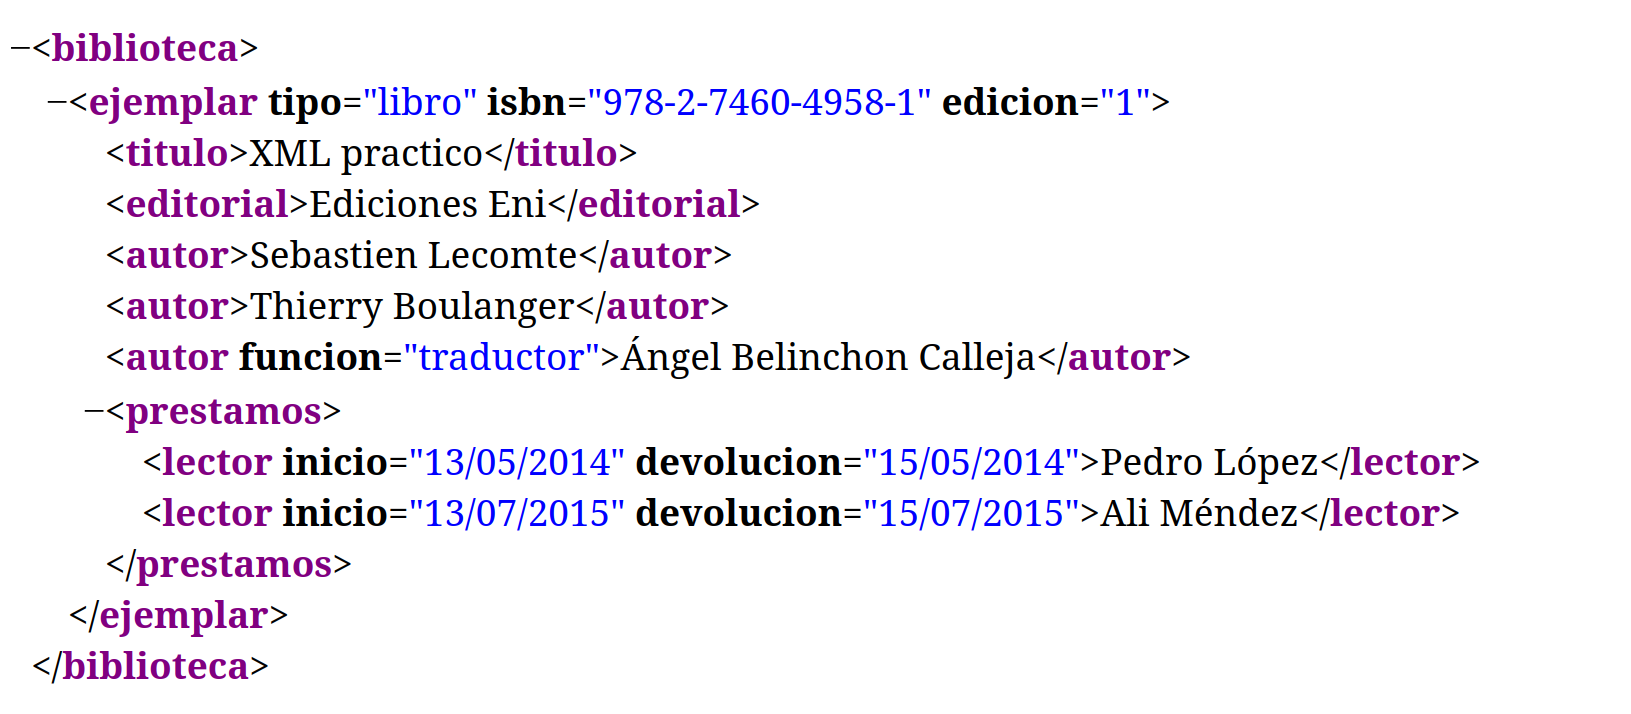
\includegraphics[scale=0.3]{ejemplo-xml.png}
    \caption{Ejemplo de XML en el navegador}
\end{figure}


% Glossary

\glsaddall
\printglossaries

% Bibliography

\newpage
\addcontentsline{toc}{chapter}{Bibliografía}
\bibliography{citas}
\bibliographystyle{unsrt}

\end{document}